%!TEX program = xelatex
%!TEX encoding = UTF-8

\documentclass[fangfont=FangSong,heifont=SimHei]{zju-thesis}
\usepackage{url}
\usepackage{lipsum} 
\usepackage{math}
\graphicspath{{./data/}}

\title{深度行人再识别学习}{浙江大学本科生毕业论文}
\author{王兴路}{3140102282}
\grade{2014 级}{信息工程}
\mentor{李英明}
\school{信息与电子工程学院}
\date{2018年6月}

\begin{document}
	\makecover
    \tableofcontents
	\begin{refsection}
	
% !TeX encoding = utf8
% !TeX root = ./main.tex

% part I
% \titleformat{\chapter}
%   {\chap}{\thechapter}{1em}{}
% \titlespacing*{\chapter}{0pt}{3.5ex plus 1ex minus .2ex}{2.3ex plus .2ex}
%
\part{毕业论文}

\chapter{引言}

\section{研究背景与意义}

\cite{small}

{\wuhao
\begin{longtable}{p{5cm}p{5cm}}
\caption{符号说明}\\
\hline
项目内容 & 特点\\
\hline
模拟& 同方差\\
\hline
\end{longtable}
}

\begin{longtable}{p{5cm}p{5cm}}
\caption{符号说明}\\
\hline
项目内容 & 特点\\
\hline
模拟& 同方差\\
\hline
\end{longtable}


\section{国内外研究现状}
\section{主要研究内容}


\chapter{基于多尺度特征融合的行人特征学习}

\section{问题概述}

行人再识别旨在学习鲁棒的特征,达到最小化类内间距和最大化类间间距的目标。
但是由于跨摄像头检索时,环境和行人姿态的各种变化,导致模型很难自发地学到具有鉴别能力的特征。
同时,由于检测器的误差,导致行人图片存在一定的空间维度偏移,即空间失配,给行人再识别带来了极大的挑战。
需要加入结构先验,才能使得模型聚焦于具有鉴别力的区域,从而获得鲁棒而紧凑的行人特征表示。 
对此,我们通过对再识别任务和数据集观察的观察,基于注意力机制,引入多尺度的结构先验。

\begin{figure}[htbp]
    \centering 
    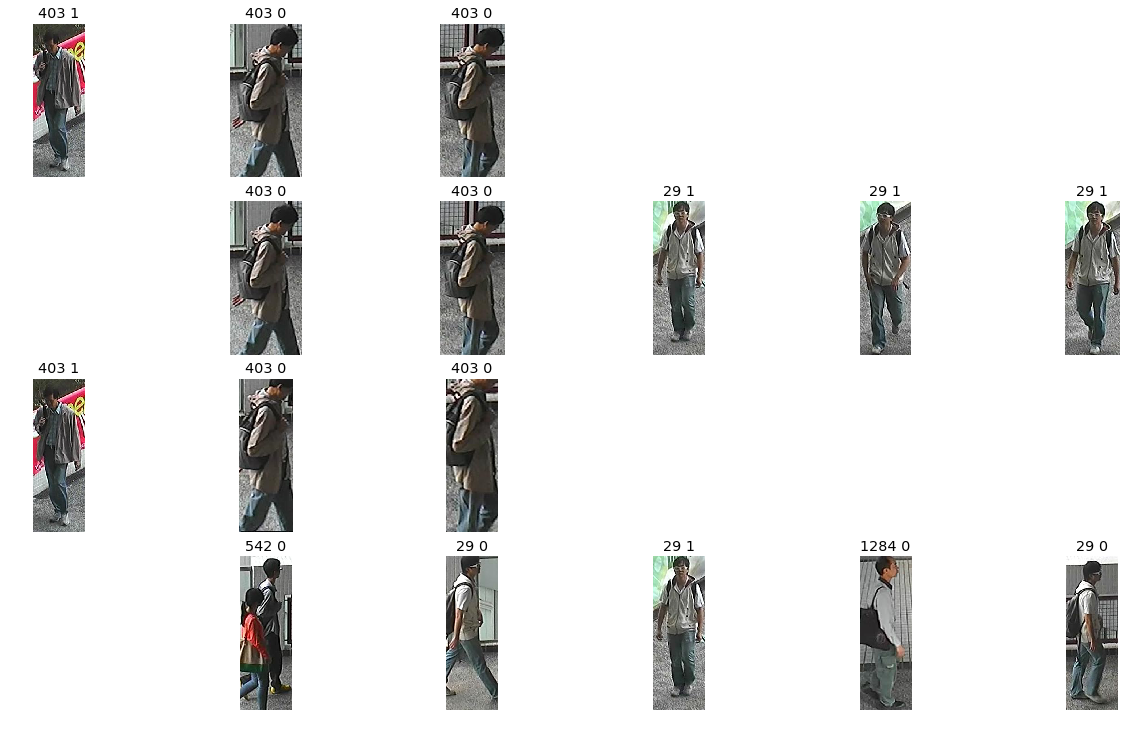
\includegraphics[width=.95\textwidth]{fig/2018-04-18-21-53-15.png}
    \caption{基准模型在手工标注数据集和行人检测器自动检测的数据集上的典型样例} \label{fig:label2det}
\end{figure}

现有工作方法的缺陷。

\misscite The Devil is in the Middle: Exploiting Mid-level Representations for Cross-Domain Instance Matching 

行人再识别可以看做将不同视角的图片映射到同一个特征空间,从而方便在统一的特征空间中进行比较。在传统的工作中,通常直接使用深度神经网络的最后一层定义统一的特征空间。但是想要应对各种变化,中层属性特征与高层语义特征十分重要。对于中层属性特征,更重要的是抽取、凝练其中重要的信息,并与高层语义表示融合。

我们提出的模型在网络结构上引入先验,从而融合高层语义特征和中层属性特征。模型包含三个模块:(1)、基于残差神经网络特征提取模块;(2)、基于注意力机制的属性特征提取模块;(3)、特征融合与度量学习模块。

对于特征融合模块,我们对中层特征采用合适的池化方式,然后与最后的语义表示通过拼接的方式形成最终的特征表示。这样的策略,从前向传播的角度看,保证了最终的表示有效包含中层属性信息;从反向传播的角度看,保证了监督信息有效反传更新中层特征,从而学到具有鉴别力的表示。基础的骨架网络也可以采用卷积神经网络结构,比如残差神经网络(ResNet)、Inception网络、Squeeze \& Extraction网络\misscite 等。

对于行人再识别任务,我们采用在ImageNet上与训练好的ResNet-50模型。该模型采用全卷积的架构,即所有的参数层都可用卷积层实现。大量的前人工作直接对最后一层卷积层(res5c)的特征进行全局池化,获得图像的表示,表示为$f^{pool5}$。可是。。。我们同时使用中间层特征来补充$f^{pool5}$。考虑到行人再识别中,姿态的多变性会导致严重的空间失配,因此图像的空间信息不是很可靠。于是我们采用。。。

\misscite Resource Aware Person Re-identification acrossMultiple Resolutions 


\section{框架设计及算法实现}


\subsection{多尺度融合结构}

\subsection{注意力模块}

\subsection{目标函数}

\section{实验设计和结果}

\subsection{数据集统计信息与评估协议}

\subsection{实验结果和比较}

\section{本章小结}


\chapter{问题的研究}

\section{问题描述}
\section{研究方法}
\section{结果验证和分析}

\chapter{结论与展望}

\section{结论}
\section{论文中出现的问题及思考}
\section{展望}

\printbibliography[heading=chapbib]
	\chapter{基于**的网络}

\section{第一节}

\section{本章小结}



	\end{refsection}
	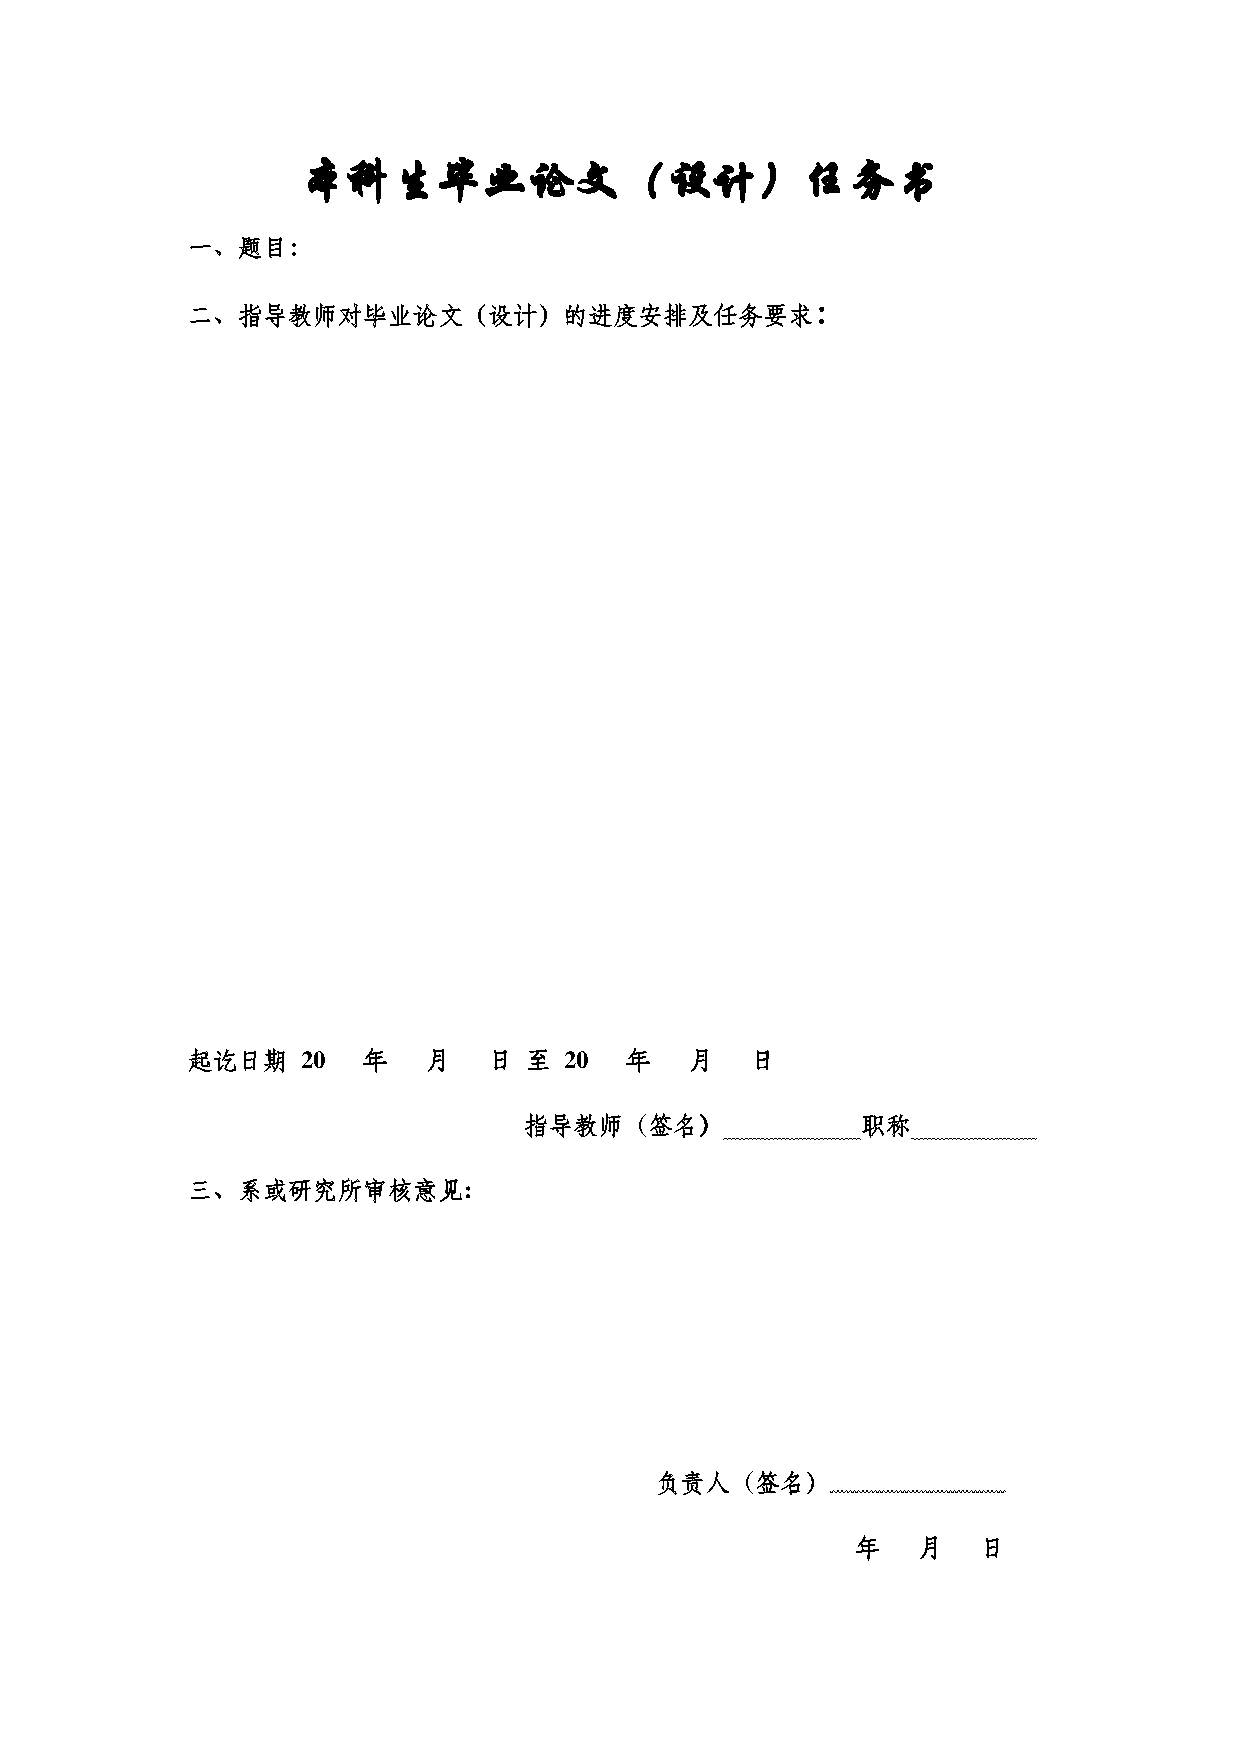
\includepdf[fitpaper=true,pages=-,pagecommand={\thispagestyle{empty}},addtotoc={
		1, alonepage, 1, 《浙江大学本科生毕业论文(设计)任务书》, task
	}]{assets/official-1-task.pdf}
	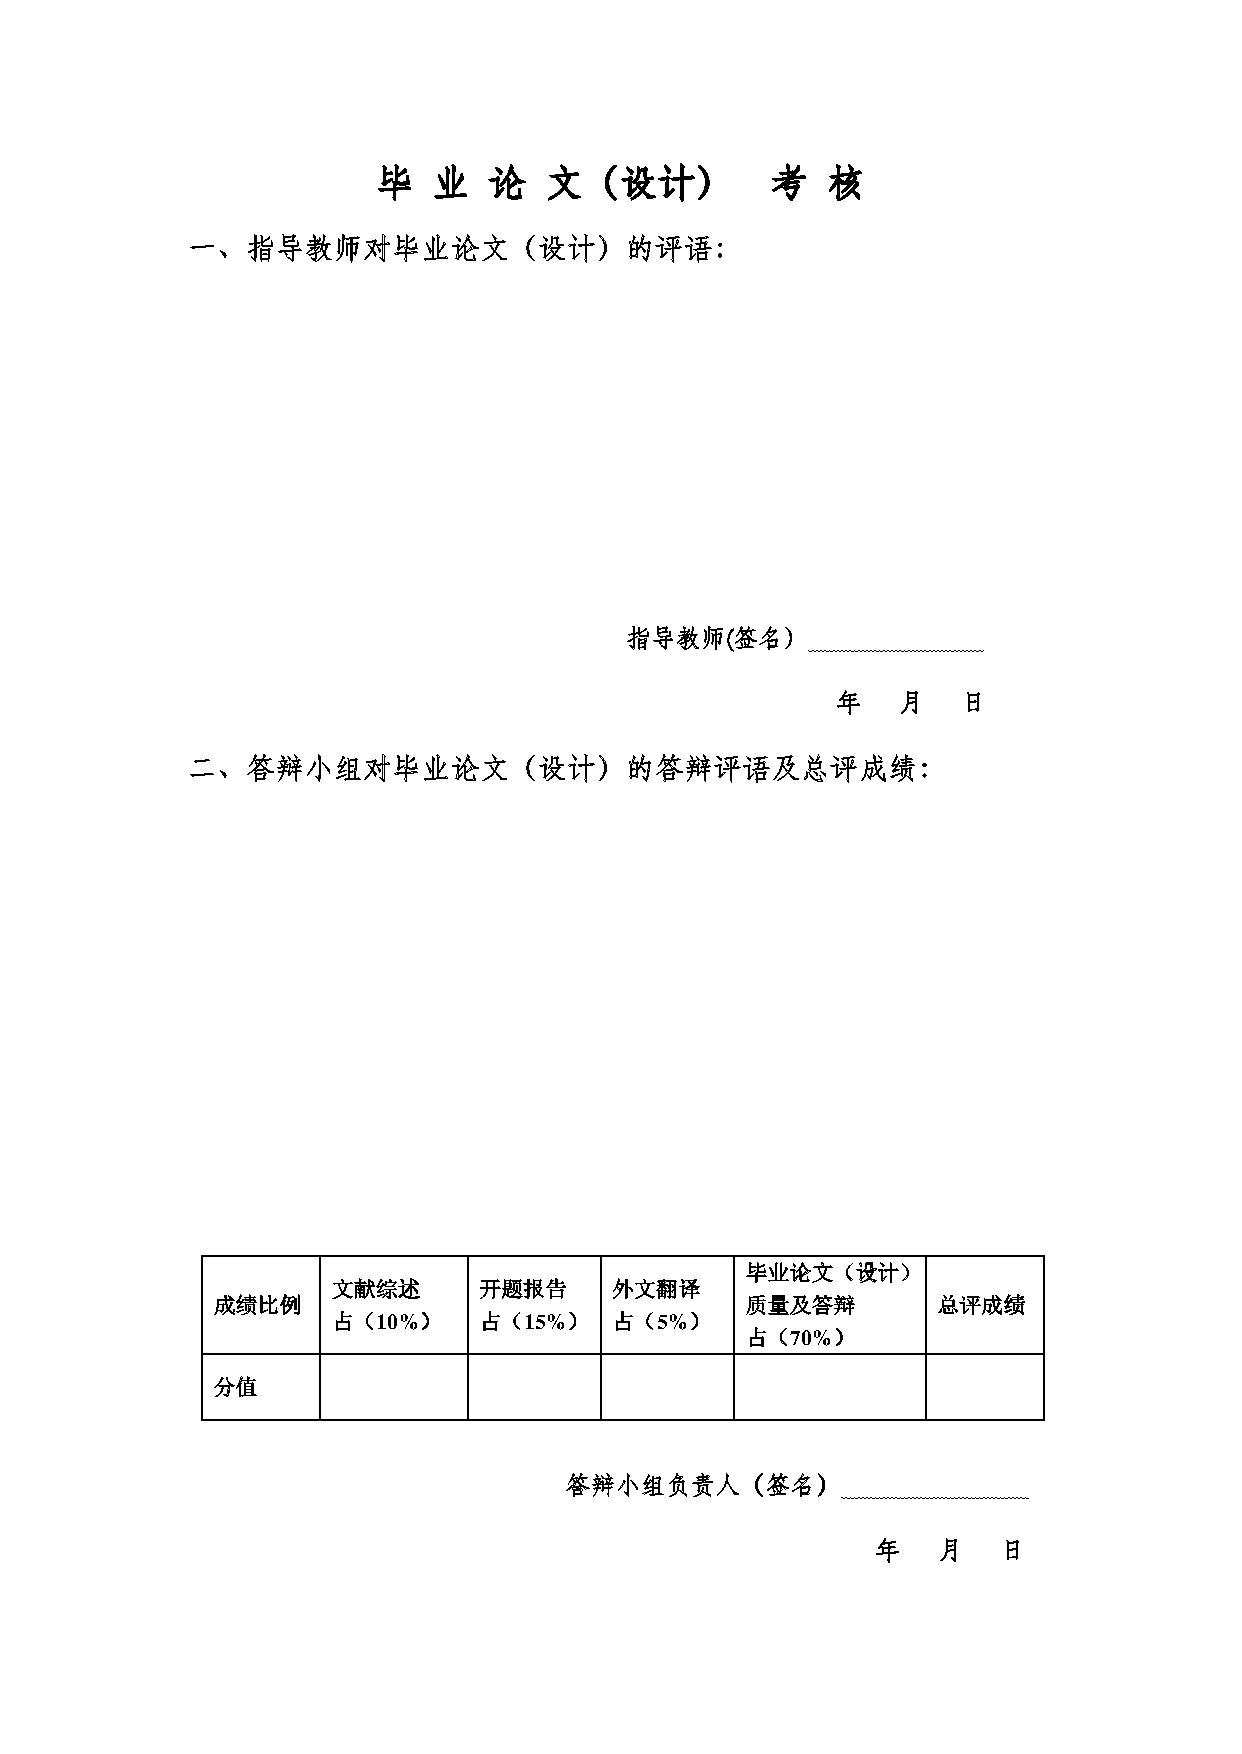
\includepdf[fitpaper=true,pages=-,pagecommand={\thispagestyle{empty}},addtotoc={
		1, alonepage, 1, 《浙江大学本科生毕业论文(设计)考核表》,assess
	}]{assets/official-11-assess.pdf}
	\part{文献综述和开题报告}
	\renewcommand\thechapter{\zhnum{chapter}、} 
	
\includepdf[fitpaper= true,pages=-,pagecommand={\thispagestyle{empty}},addtotoc={
		1, alonepage, 1, 文献综述和开题报告封面, cover,
		1, alonepage, 1, 指导教师对文献综述和开题报告具体内容要求, cover,
		1, contabpage, 1, 目录,con,
		1, chapter, 1, 文献综述,s1,
		5, chapter, 1, 开题报告,s2,
		6, chapter, 1, 外文翻译,s3, 
		7, chapter, 1, 外文原文,s4,
		8, alonepage, 1, 《浙江大学本科生文献综述和开题报告考核表》,s5}]{../proposal/main.pdf}
\end{document}